%!TEX root = ../tesi.tex

\chapter{Gestione dei dati nello Shadow Framework 2.0}
\label{ch:gestionedati}

% TODO: ampliare l'introduzione
La gestione dei dati \`e un compito molto importante all'interno del framework. Attraverso l'utilizzo di un layer di gestione dati astratto, ogni mudulo del framework pu\`o essere salvato e caricato da file o trasferito attraverso un qualsiasi flusso di dati.
In questo capitolo viene presentata l'astrazione utilizzata dallo Shadow Framework nella gestione dei dati, le funzionalit\`a messe a disposizione ed i principali package e moduli coinvolti.

\section{Dati grafici}
\label{sec:dati grafici}
Data la natura del framework la tipologia di dato pi\`u critica e importante \`e quella che descrive le informazioni grafiche. 
L'unit\`a base di ogni dato di tipo grafico \`e l'\texttt{SFDataAsset}, questa \`e una classe astratta generica che serve ad automatizzare il processo di costruzione dei dati e inizializzazione degli stessi nella memoria grafica. Questo processo non pu\`o per\`o essere effettuato in qualsiasi momento, ma deve essere correttamente sincronizzato con il processo di rendering della pipeline del framework, in caso contrario i dati potrebbero venir alterati durante il disegno della scena portando ad effetti inaspettati.

\begin{figure}
\begin{center}
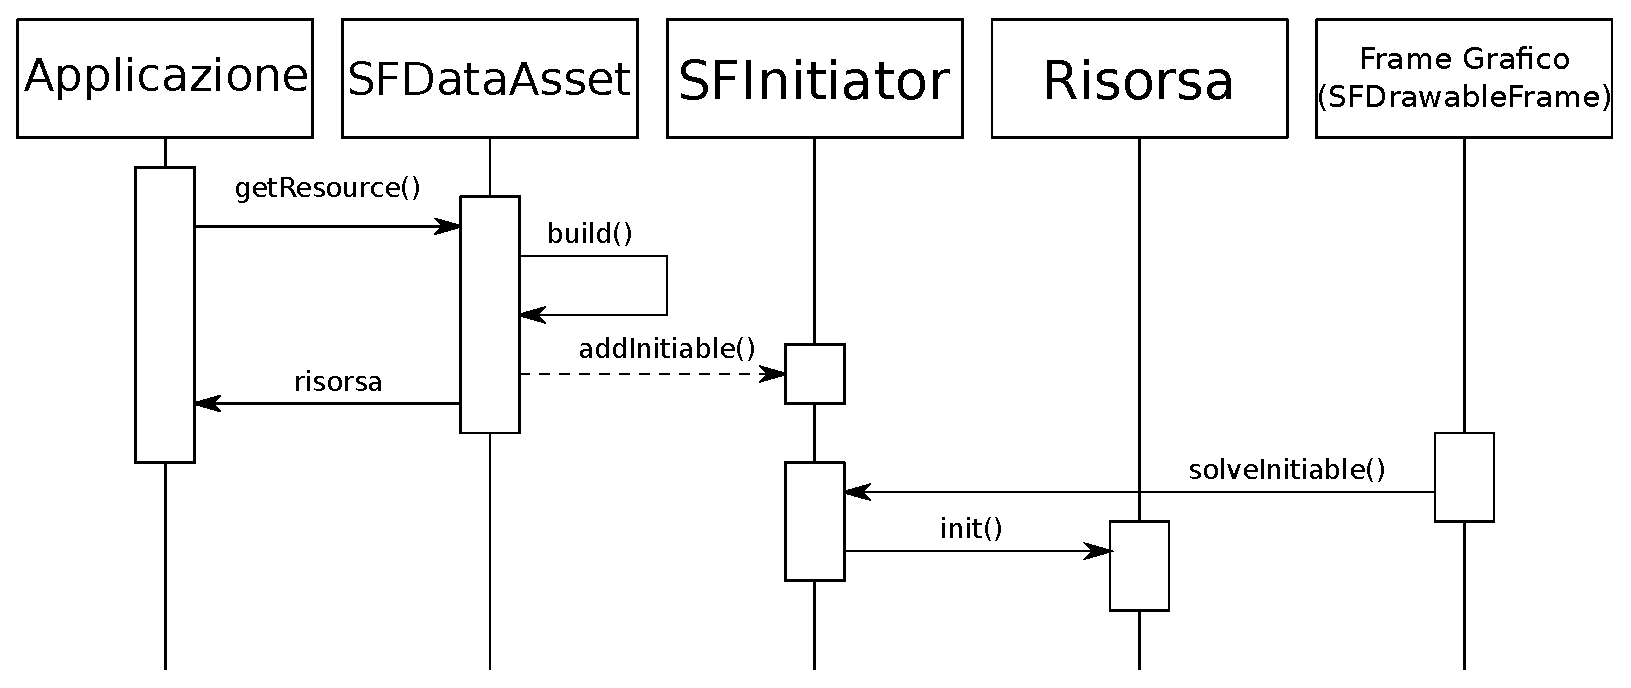
\includegraphics[width=\textwidth]{Immagini/sequenzaDataAsset}
\caption[Diagramma della fase di costruzione di un SFDataAsset.]{Diagramma di sequenza della fase di costruzione di un SFDataAsset.\label{f:seqdataasset}} 
\end{center} 
\end{figure}

Il diagramma della figura \ref{f:seqdataasset} mostra la sequenza di operazioni necessarie affinch\'e le informazioni del DataAsset grafico vengano costruite correttamente e inizializzate nella memoria grafica in modo sincrono con il processo di rendering, gestito dal frame grafico \textbf{SFDrawableFrame}.
Partendo da in alto a sinistra l'applicazione richiede la risorsa all'\texttt{SFDataAsset}, questo la costruisce con il metodo \texttt{build()} e notifica all'\texttt{SFInitiator} che la risorsa necessita di essere inizializzata nella memoria grafica tramite la chiamata \texttt{addInitiable()}, dopo di che il riferimento alla risorsa viene restituito all'applicazione.
Il processo di rendering chiede all'Initiator, ciclicamente e nel momento opportuno, di inizializzare nella memoria grafica tutti i DataAsset che sono in attesa di farlo. L'Initiator richiama allora il metodo \texttt{init()} di tutte le risorse in attesa di inizializzazione.
Questo procedimento assicura che tutte le risorse necessarie al processo di rendering siano inizializzate correttamente prima di essere usate.

\begin{figure}
\begin{center}
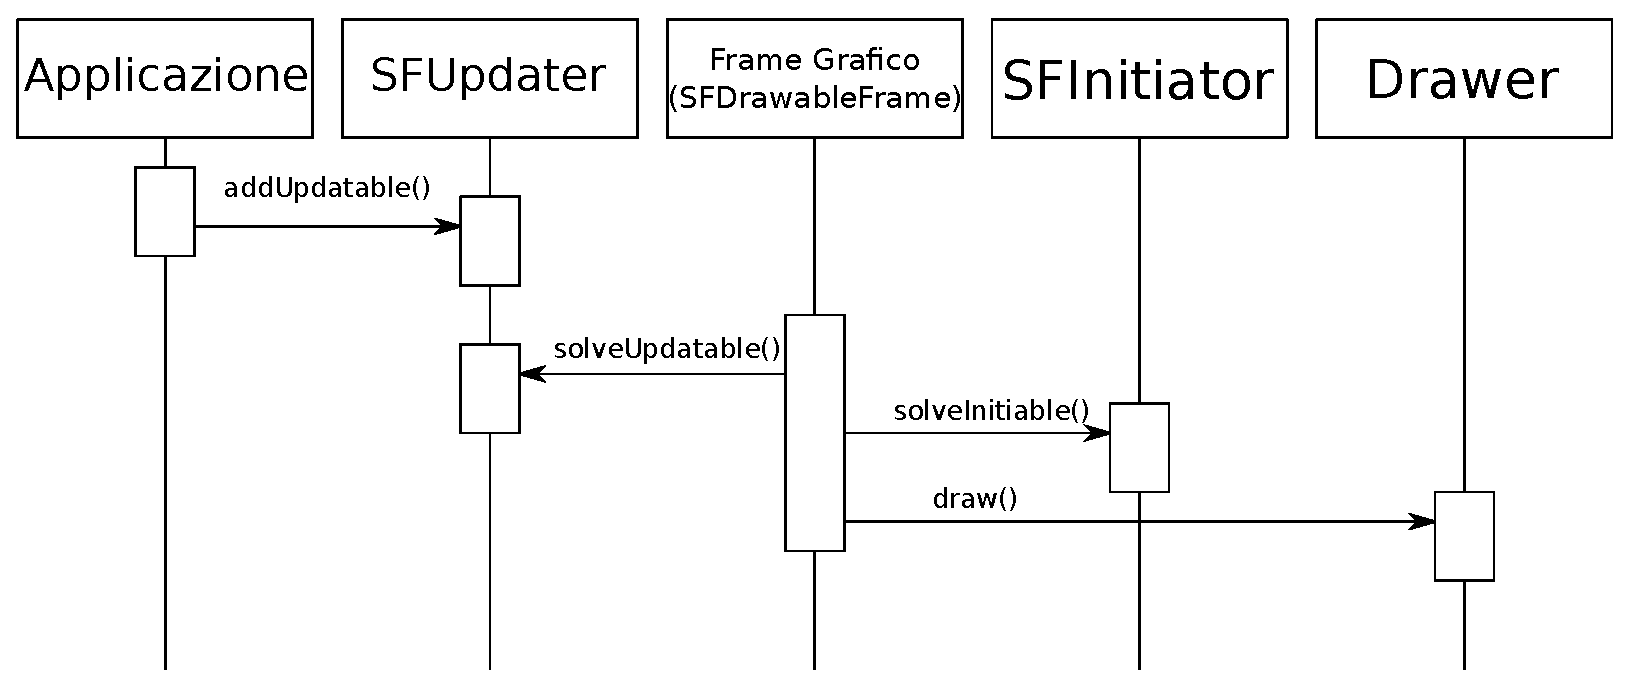
\includegraphics[width=\textwidth]{Immagini/sequenzaUpdatable}
\caption{Diagramma di sequenza dell'update dei dati.\label{f:sequpdate}} 
\end{center} 
\end{figure}

Internamente al framework esiste inoltre un meccanismo di sincronizzazione analogo pensato per effettuare un aggiornamento dei dati che sono gi\`a stati inizializzati. Questo sistema si basa sull'utilizzo di un Updater che si comporta analogamente a quanto visto con l'Initiator. Il diagramma di sequenza in figura \ref{f:sequpdate} mostra la sequenza temporale di un update dei dati: quando l'applicazione necessita di aggiornare i dati grafici passa all'\texttt{SFUpdater} un metodo di callback che contiene al suo interno tutte le operazioni da eseguire durante l'aggiornamento.
Il frame grafico che esegue ciclicamente il rendering, prima di effettuarlo, chiede all'Updater e poi all'Initiator di risolvere tutte le operazioni che hanno in sospeso. L'ordine in questo caso \`e di fondamentale importanza perch\'e l'aggiornamento dei dati potrebbe comportare l'aggiunta di DataAsset che necessitano di essere inizializzati. Questo sistema \`e stato inizialmente pensato per gli aggiornamenti delle animazioni, ma pu\`o essere sfruttato per qualsiasi operazione critica di aggiornamento dei dati.

\section{L'astrazione della gestione dati}
\label{sec:astrazione}
All'interno di un'applicazione \ac{SF} l'unit\`a base di dati pu\`o essere identificata con quello che viene definito SFDataset la cui spiegazione verr\`a dettagliata nel paragrafo \ref{sub:sfdataset}. Con Dataset si identifica quasi ogni tipo di dato, sia grafico che non, utilizzato all'interno del framework: un \texttt{SFDataAsset} ad esempio \`e una sottoclasse di \texttt{SFDataset}.
La gestione dei dataset viene effettuata mediante un meccanismo centralizzato: ogni applicazione in esecuzione possiede un'istanza di SFDataCenter, la quale \`e un oggetto \textit{Singleton} che realizza un \textit{Bridge}
tra l'astrazione di reperimento dati e la sua implementazione concreta\footnote{Con \textit{Singleton} e \textit{Bridge} si intendono i design pattern omonimi descritti pi\`u in dettaglio nell'appendice \ref{a:designpatterns}}.
Ogni componente pu\`o accedere al DataCenter per richiedere operazioni sui Dataset di interesse, come la lettura o la scrittura da uno stream specifico, la richiesta di una particolare istanza di un Dataset, identificata per nome, o la richiesta di una nuova istanza di Dataset, identificata per tipo.
L'oggetto Singleton espone queste funzionalit\`a traducendole internamente con chiamate ad una \textit{factory} concreta\footnote{Si fa riferimento al pattern di programmazione \textit{Abstract Factory} descritto nella sezione \ref{sub:abstractfactory}.}
di Dataset e ad una istanza dell'interfaccia SFIDataCenter, creando un'astrazione su come vengano effettivamente costruiti e reperiti i Dataset, come mostrato nelle immagini \ref{f:datacenterfactory} e \ref{f:datacenterimplementation}.
La factory concreta deve essere un'implementazione dell'interfaccia SFAbstractDatasetFactory in grado di istanziare, leggere o scrivere ogni tipo di Dataset utilizzato dall'applicazione.
L'istanza dell'interfaccia SFIDataCenter tiene traccia dei Dataset istanziati con nome, restituendone un riferimento a chi ne fa richiesta attraverso la chiamata a funzioni di callback.

\begin{figure}
\begin{center}
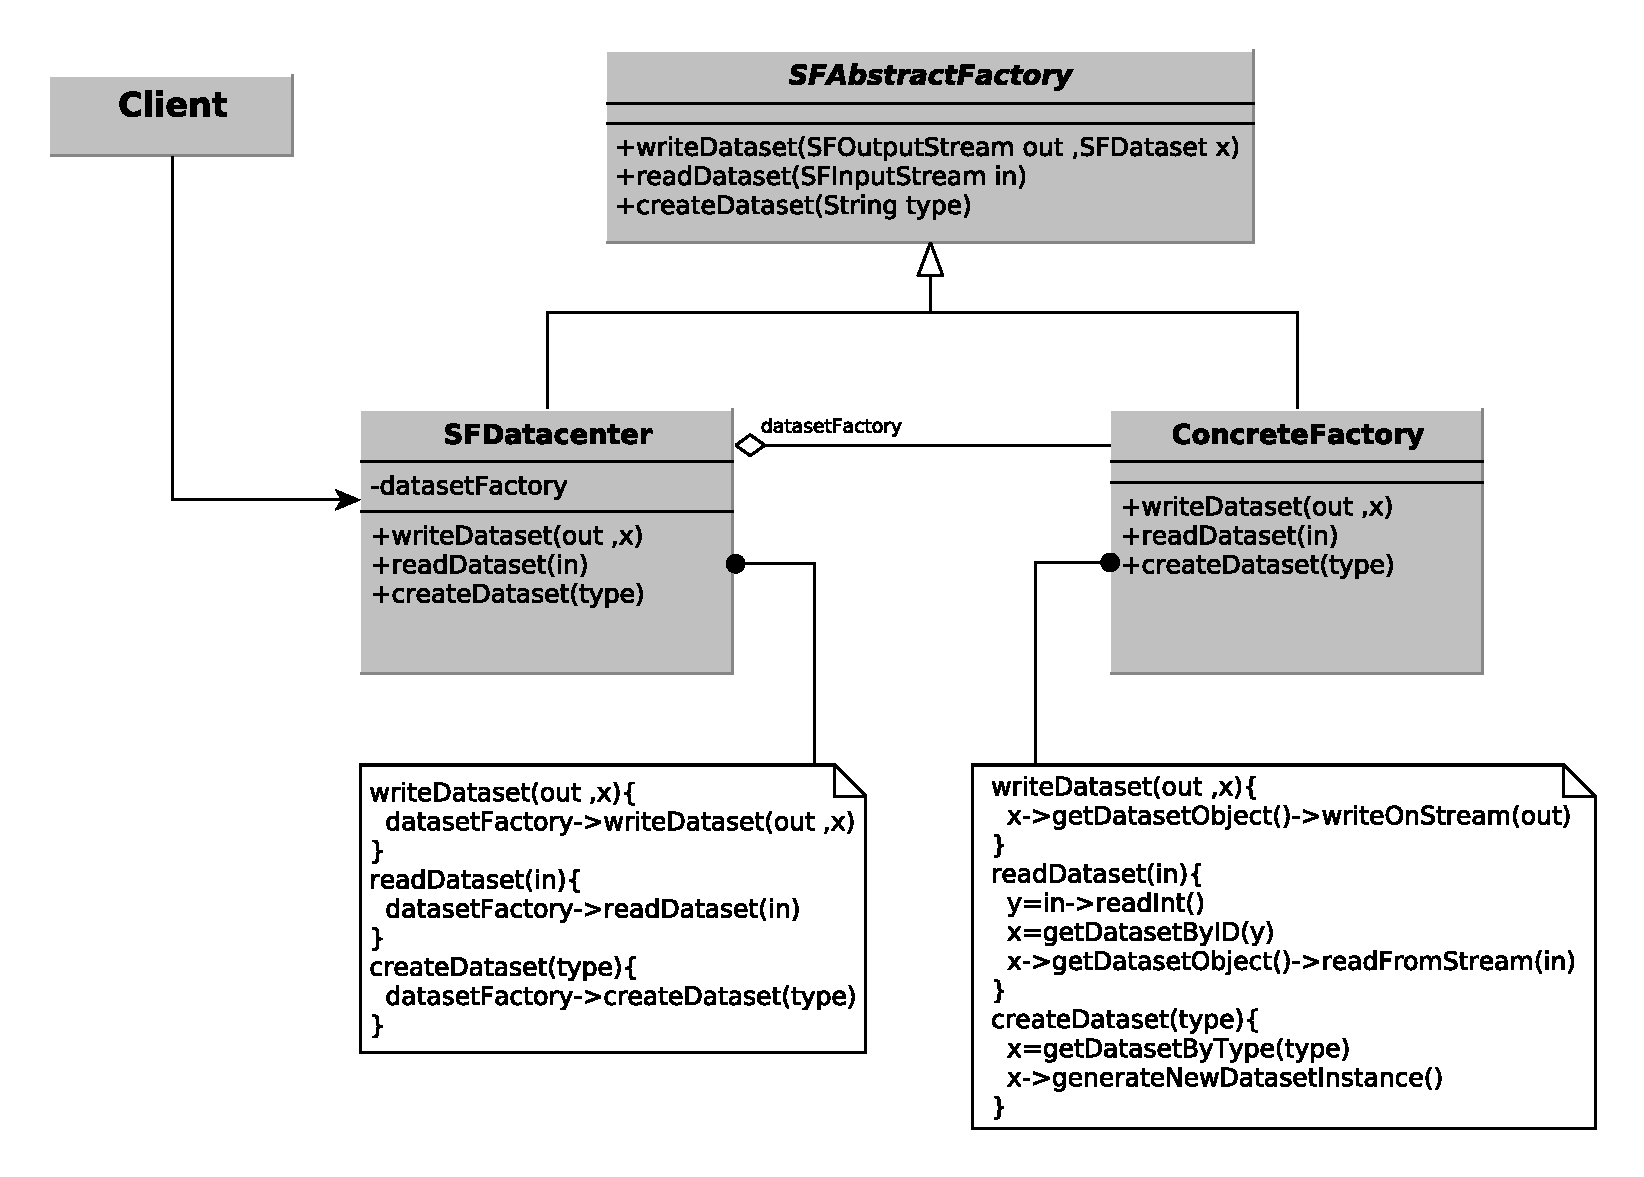
\includegraphics[width=\textwidth]{Immagini/DataCenterfactory}
\caption[Bridge composto da SFDataCenter e SFAbstractFactory.]{Diagramma del Bridge composto da SFDataCenter e da un'istanza concreta di SFAbstractFactory.\label{f:datacenterfactory}} 
\end{center} 
\end{figure}
\begin{figure}
\begin{center}
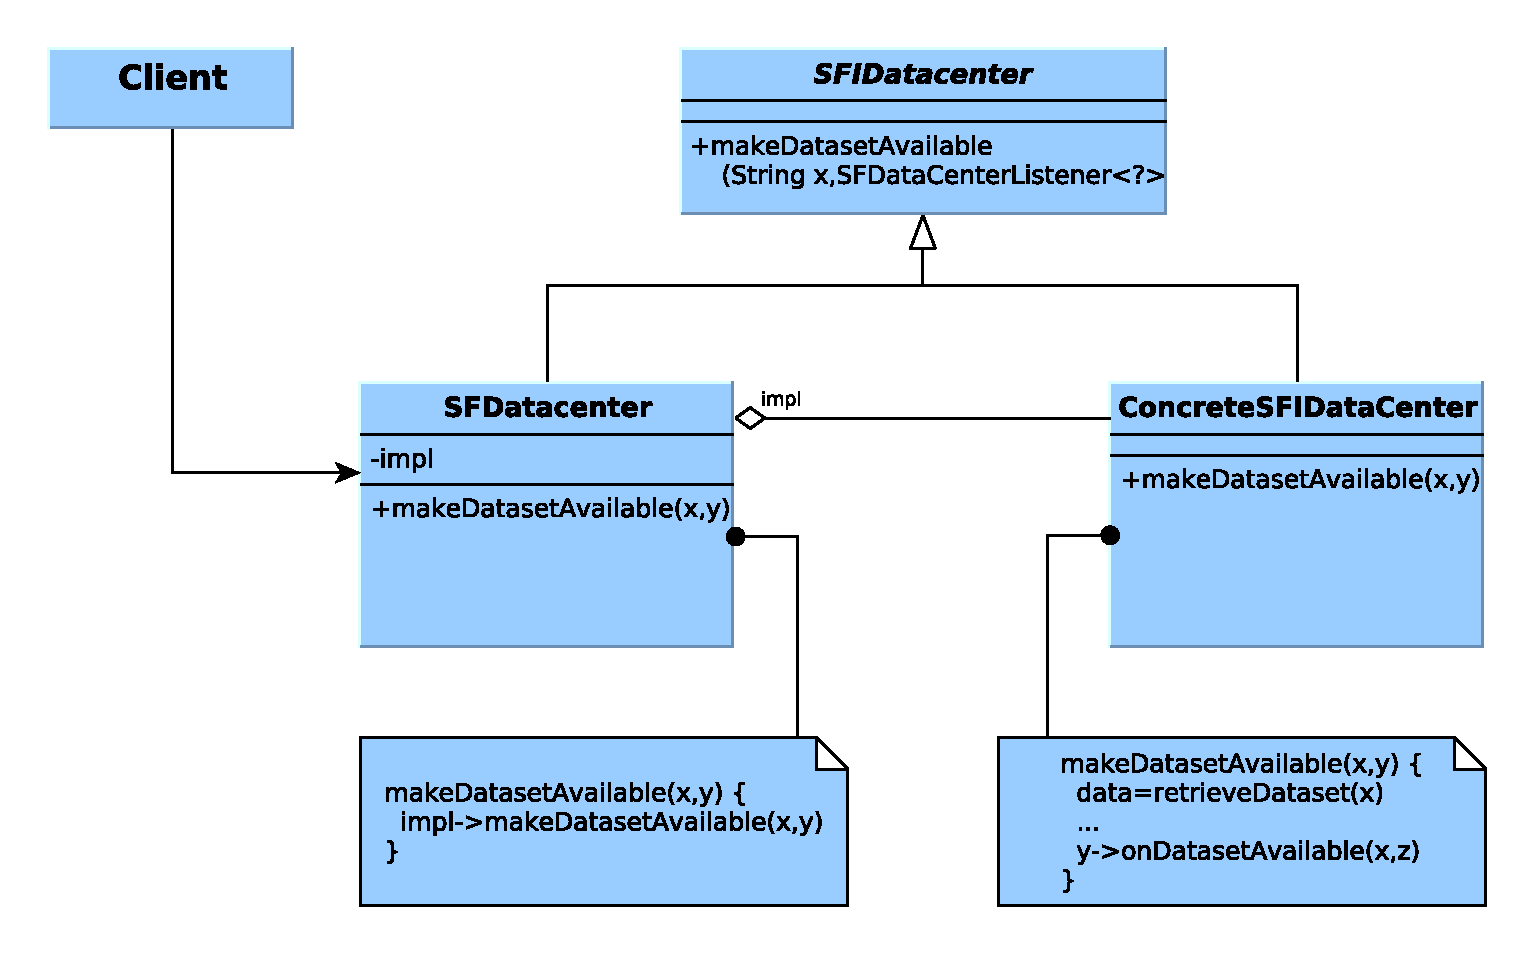
\includegraphics[width=\textwidth]{Immagini/DataCenter}
\caption[Bridge composto da SFDataCenter e SFIDataCenter.]{Diagramma del Bridge composto da SFDataCenter e da un'istanza concreta di SFIDataCenter.\label{f:datacenterimplementation}} 
\end{center} 
\end{figure}

\section{Il package \texttt{shadow.system.data}}
\label{sec:shadow_system_data}
Questo package contiene una serie di classi ed interfacce su cui si basa l'astrazione dei dati del framework.

\subsection{SFInputputStream e SFOutputStream}
\label{sub:sfinoutstream}
Queste interfacce definiscono le operazioni necessarie che uno stream di input o di output deve implementare affinch\'e sia possibile leggere o scrivere su di esso dei DataObject e insieme costituiscono un elemento molto importante per l'estendibilit\`a del framework sui dati. Su di esse si basa infatti l'astrazione che i dati utilizzano per completare le operazioni di lettura e scrittura. Utilizzando la medesima interfaccia di astrazione \`e possibile far comunicare tra loro anche implementazioni diverse del framework.

\subsection{SFDataObject}
\label{sub:sfdataobject}
Uno dei moduli principali del package \`e \texttt{SFDataObject}, che rappresenta un'interfaccia con funzionalit\`a di base comuni ad ogni oggetto che contiene dati. 
Ogni oggetto di questo tipo pu\`o perci\`o:
\begin{itemize}
	\item essere scritto su di un \texttt{SFOutputStream};
	\item essere letto da un \texttt{SFInputStream};
	\item essere clonato;
\end{itemize}
I DataObject si basano sul \textit{Composite Pattern} (\ref{sub:composite}): possono essere semplici o contenere un insieme di oggetti figli. Il fatto che sia gli oggetti complessi che quelli semplici condividano la stessa interfaccia permette di trattarli in maniera uniforme. Un oggetto contenitore dovr\`a semplicemente richiamare lo stesso metodo di interfaccia per tutti gli oggetti figli i quali, se oggetti semplici, hanno la responsabilit\`a di implementare l'algoritmo per leggere o scrivere se stessi da uno stream.

Tutti i componenti SF utilizzano dei DataObject per incapsulare i dati in modo che questi ultimi possano essere letti e scritti utilizzando stream appropriati.

\begin{figure}
\begin{center}
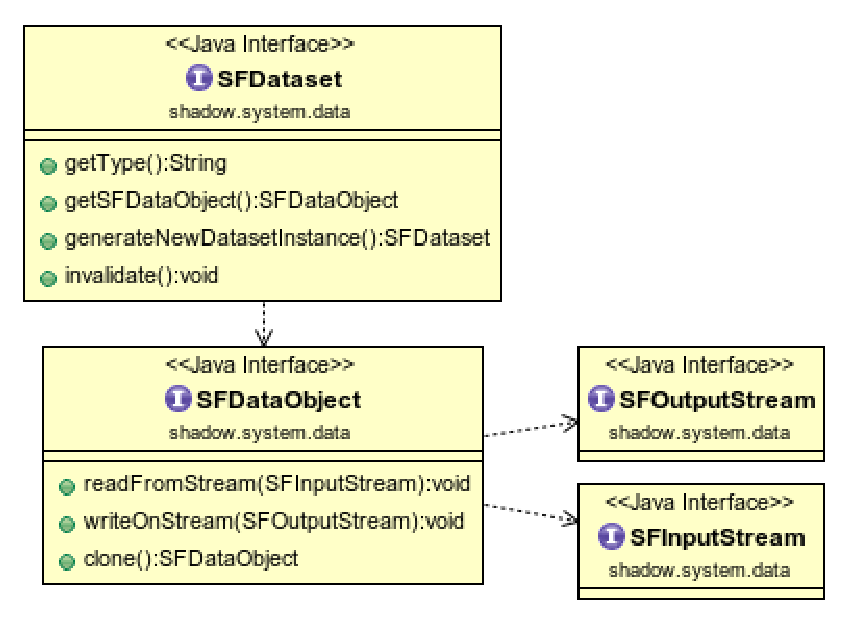
\includegraphics[width=11cm]{Immagini/relazione-dataset-dataobject-stream}
\caption[Relazioni tra le classi di gestione dati.]{Diagramma della relazione tra le classi SFDataset, SFDataObject, SFInputStream e SFOutputStream.\label{f:dataset-dataobj-stream}} 
\end{center} 
\end{figure}

\subsection{SFDataset}
\label{sub:sfdataset}
Un altro modulo importante per la gestione dei dati \`e \texttt{SFDataset}. Un Dataset \`e un oggetto che contiene un DataObject e informazioni sul proprio tipo, rappresentato tramite una stringa.
Da come si pu\`o intuire dalla figura \ref{f:dataset-dataobj-stream} il DataObject viene sfruttato dal Dataset per incapsulare i suoi dati interni ed incorporarne le funzionalit\`a di lettura e scrittura.
L'interfaccia SFDataset definisce un'interfaccia per oggetti di questo tipo, la quale consente di accedere al nome del tipo specifico, al DataObject contenuto e di creare una nuova istanza delle stesso tipo.
A loro volta i Dataset possono essere incapsulati in un DataObject usando un oggetto \texttt{SFDatasetObject}.

\subsection{SFAbstractDatasetFactory}
\label{sub:sfabstractdatasetfactory}
Questa interfaccia definisce le operazioni base richieste ad una DatasetFactory. Le operazioni consistono in:
\begin{itemize}
	\item lettura/scrittura di un Dataset da uno stream;
	\item creazione di una nuova istanza di un Dataset specificato per tipo.
\end{itemize}

\subsection{SFIDataCenter}
\label{sub:sfidatacenter}
L'interfaccia \texttt{SFIDataCenter} fornisce l'astrazione di una Mappa di Dataset identificati attraverso il proprio nome.
Grazie ad essa possiamo chiedere ad un oggetto che la implementa di recuperare un Dataset specifico.
Quest'oggetto non deve restituire direttamente il Dataset recuperato, ma deve farlo attraverso un meccanismo di callback ad una implementazione dell'interfaccia \texttt{SFDataCenterListener} passata come parametro, nel momento in cui il dato \`e disponibile.

\begin{figure}
\begin{center}
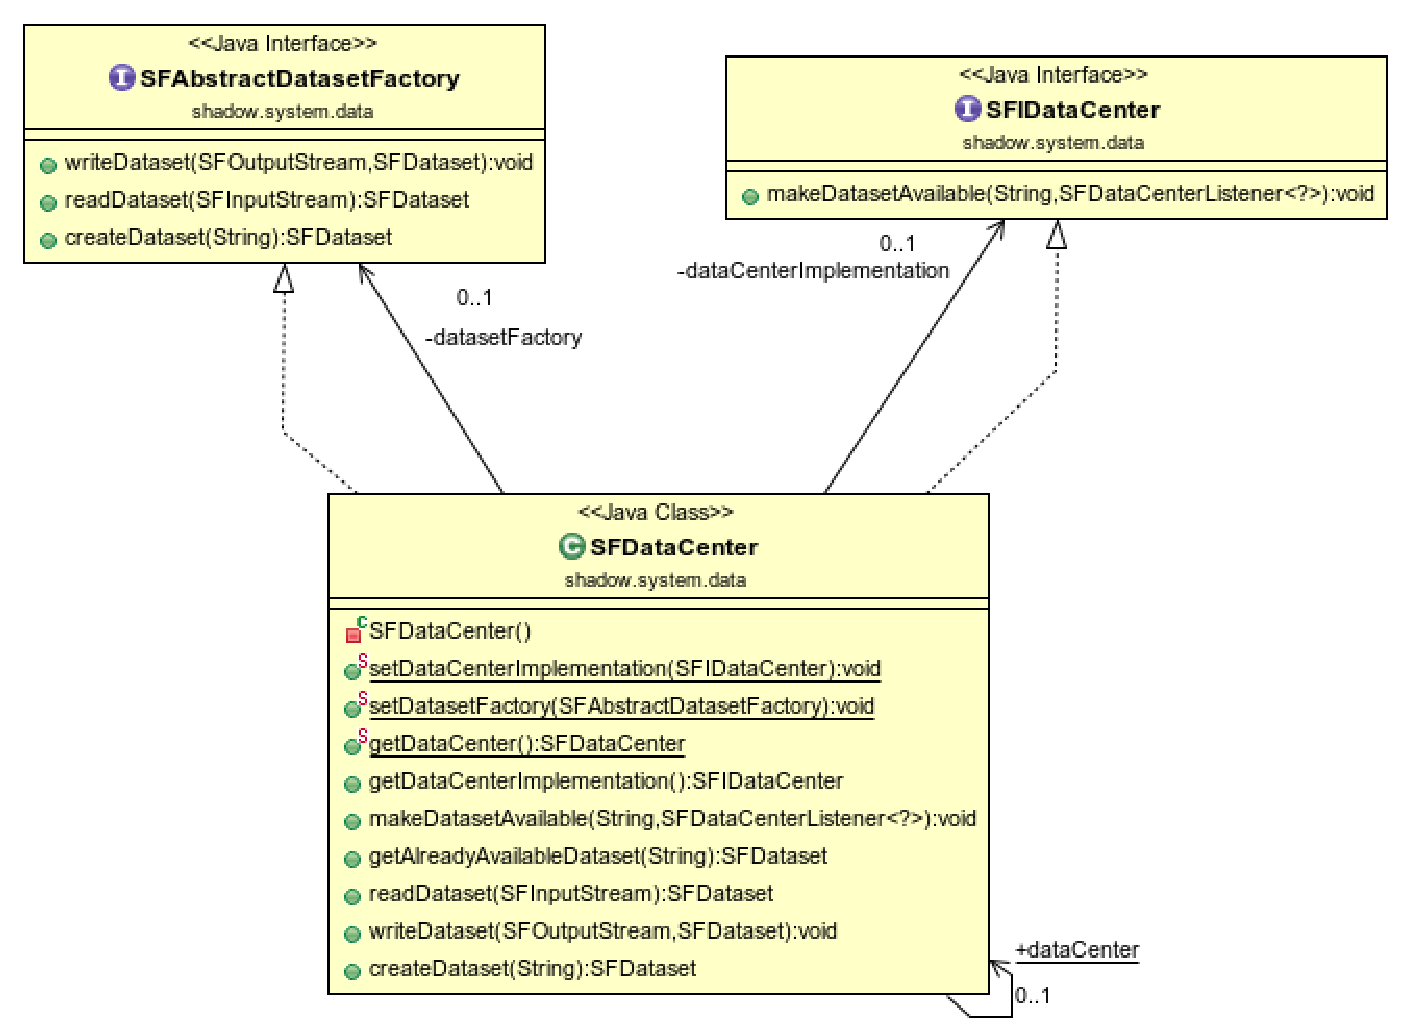
\includegraphics[width=\textwidth]{Immagini/DataCenterBridge}
\caption[Relazione tra le classi del bridge SFDataCenter.]{In questo diagramma viene mostrata la relazione tra le classi SFDataCenter, SFIDataCenter e SFAbstractDatasetFactory. Da notare che SFDataCenter \`e una classe Singleton in quanto contiene una istanza statica di se stessa (l'istanza dataCenter sottolineata) e possiede un costruttore privato (evidenziato in rosso). Inoltre, in riferimento alla sezione \ref{sub:bridge}, si pu\`o notare come SFDataCenter realizzi un Bridge sia con SFIDataCenter che con SFAbstractDatasetFactory \label{f:datacenterbridge}} 
\end{center} 
\end{figure}

\subsection{SFDataCenterListener}
\label{sub:sfdatacenterlistener}
Questa interfaccia definisce la callback che un componente deve implementare per effettuare una richiesta al DataCenter.
La callback viene richiamata quando il Dataset richiesto \`e pronto.

\subsection{SFDataCenter}
\label{sub:sfdatacenter} 
% TODO: evitare di ripetere quanto detto in sec:astrazione
Il \textbf{DataCenter} \`e il nodo fondamentale della gestione dei dati all'interno del framework. 

\'E un oggetto \textit{Singleton} (\ref{sub:singleton}) a cui le applicazioni accedono per richiedere i Dataset di cui hanno bisogno. Questa classe utilizza anche il pattern \textit{Bridge} (\ref{sub:bridge}), fornendo un'astrazione su come i dati sono effettivamente reperiti.

Per poter funzionare, al DataCenter deve essere fornita un'implementazione per:
\begin{itemize}
	\item \texttt{SFAbstractDatasetFactory}
	\item \texttt{SFIDataCenter}
\end{itemize}

Come precedentemente esposto, l'implementazione di \texttt{SFAbstractDatasetFactory} deve essere essere una factory in grado di generare istanze di tutti i tipi di Dataset necessari all'applicazione.

Questo tipo di astrazione permette di separare la logica di utilizzo del Dataset da quella di come esso viene reperito, consentendo ad una applicazione di usare dati locali o dati di rete semplicemente cambiando l'implementazione di \texttt{SFIDataCenter}.

\subsection{SFObjectsLibrary}
\label{sub:sfobjectslibrary}
\'E usata per memorizzare un set di Dataset ed al suo interno ogni elemento \`e identificato tramite un nome univoco.
Un \texttt{SFObjectsLibrary} \`e a sua volta un Dataset, cos{\`\i} che un ObjectsLibrary possa essere contenuta in altre ObjectsLibrary.
\'E possibile, ad esempio, utilizzare una ObjectsLibrary all'interno di implementazione di \texttt{SFIDataCenter} per creare una mappa di Dataset necessari al funzionamento di un'applicazione.

\section{Classi di utilit\`a per il layer dati}

\subsection{SFLibraryreference}
\label{sub:sflibraryreference}
Un LibraryReference \`e un DataObject che pu\`o essere usato da qualsiasi componente per avere un riferimento ad un Dataset memorizzato in una libreria. Viene utilizzato all'interno di DataObject o di Dataset per non avere istanze doppie dello stesso dato.

\subsection{SFGenericDatasetFactory}
\label{sub:sfgenericdatasetfactory}
Questa classe di utilit\`a consiste in una implementazione concreta di default dell'interfaccia \texttt{SFAbstractDatasetFactory}.
Per consentire il riutilizzo del codice questa implementazione sfrutta il meccanismo di \textit{factory con prototipo}: una \textit{factory} pura deve avere un metodo specifico per ogni tipo di oggetto che pu\`o istanziare, questo rende predeterminato il numero di tipi istanziabili e rende necessario modificare il codice, aggiungendo un nuovo metodo, quando si desidera modificare le capacit\`a della \textit{factory}.
Sfruttando invece il meccanismo dei prototipi non si ha un numero predeterminato di tipi istanziabili poich\'e diviene configurabile: attraverso un metodo apposito vengono passati come parametro i prototipi di ogni oggetto che la \textit{factory} deve essere in grado di creare.
Questo sposta la responsabilit\`a dalla conoscenza di come ogni singolo oggetto deve essere allocato sull'oggetto stesso, evitando di modificare la \textit{factory} ogni volta che un oggetto viene alterato.
Nel concreto la \texttt{SFGenericDatasetFactory} \`e resa configurabile tramite l'aggiunta di un metodo addSFDataset() che consente di generare, in un oggetto GenericDatasetFactory, un elenco di Dataset istanziabili.
Quando verranno chiamati i metodi dell'interfaccia SFAbstractDatasetFactory sull'oggetto GenericDatasetFactory diviene sufficiente richiamare il metodo \texttt{generateNewDatasetInstance()} del Dataset del tipo richiesto.